\documentclass[10pt,letterpaper]{article}
\usepackage{tools}
\usepackage{enumitem}
%\settextfont{B Nazanin}
\usepackage{lipsum}
\setlength{\parskip}{3mm}
\setlength{\parindent}{0mm}
\begin{document}
\Large
\begin{center}
In the name of beauty

3rd problem set of ComNet course
\hl
\end{center}
Q1)
\begin{enumerate}[label=\alph*-]
\item
False. Trasport and network layer protocols provide logical communication between processes running at different hosts and hosts, respectively.
\item
False. Only UDP packets are called datagrams. Another standard reserves the term segment for all Transport layer packets.
\item
False. TCP ensures that the transmitted packets would finally reach their destination as well as it guarantees the order of the packets.
\item
False. 
The IP service model does not even guarantee that a single packet would finally reach its destination. This is due to the upper layers.
%\item
%Cookies are used to keep track of user IDs in a stateless HTTP server.
%\item
%Link-layer switches are typically capable of processing the packets up to the layer 3.
%\item
%SMTP and FTP are examples of layer 1 protocols while TCP is a transport layer protocol.
%\item
%API is a set of rules 
%\item
%For economical reasons, exploiting optical fibers is not recommended in long-haul network
\end{enumerate}

Q2)
\begin{enumerate}[label=\alph*-]
\item
IP is an unreliable service because using it, no packet is presumed to arrive at the receiver. However, mechanisms such as alerting and informing the sender for every packet it transmitted and successfully received by the receiver and using TIMEOUTs would be implemented in TCP to make sure no pachet has been ignored.
\item
They are used to address the processes to which the packets should be forwarded. Ignoring them would cause the destination become unreachable.
\end{enumerate}

Q3) Assuming A, B and S would choose port numbers of 5000,6000 and 25 respectively:
\begin{enumerate}[label=\alph*-]
\item
\[
\begin{split}
&\text{
\# Source Port = 5000\quad,\quad \# Dest. Port = 25
}
\\&\text{
Source IP Addr. = A\quad,\quad Dest. IP Addr. = S
}
\end{split}
\]
\item
\[
\begin{split}
&\text{
\# Source Port = 6000\quad,\quad \# Dest. Port = 25
}
\\&\text{
Source IP Addr. = B\quad,\quad Dest. IP Addr. = S
}
\end{split}
\]
\item
\[
\begin{split}
&\text{
\# Source Port = 25\quad,\quad \# Dest. Port = 5000
}
\\&\text{
Source IP Addr. = S\quad,\quad Dest. IP Addr. = A
}
\end{split}
\]
\item
\[
\begin{split}
&\text{
\# Source Port = 25\quad,\quad \# Dest. Port = 6000
}
\\&\text{
Source IP Addr. = S\quad,\quad Dest. IP Addr. = B
}
\end{split}
\]
\item
Yes, since the sockets are indeed different because of distinct IP addresses.
\item
No if it is not presumed that the server could handle two concurrent and independent connections on a same socket.
\end{enumerate}

Q4)
%Consider the following Figure. What are the source and destination port values in the segments
%flowing from the server back to the clients’ processes? What are the IP
%addresses in the network-layer datagrams carrying the transport-layer segments?
%\begin{figure}[ht]
%\centering
%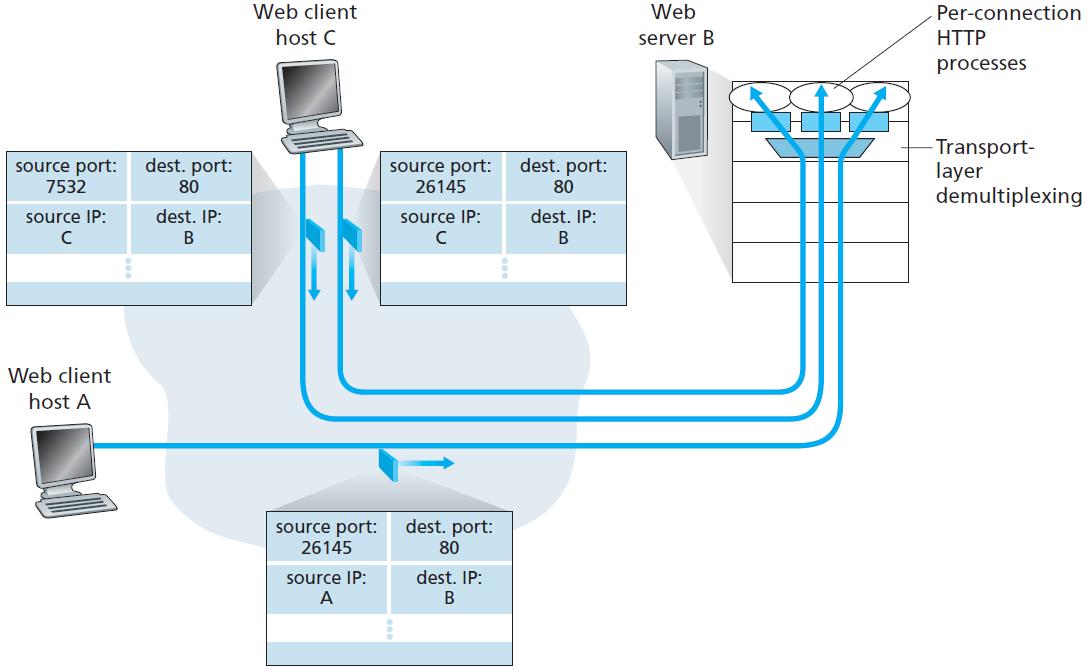
\includegraphics[width=180mm]{simnet}
%\end{figure}
\[
\begin{split}
&\text{
From B to A : \# Dest. Port = 26145\quad,\quad Dest. IP Addr. = A
}
\\&\text{
From B to C (1) : \# Dest. Port = 7532\quad,\quad Dest. IP Addr. = C
}
\\&\text{
From B to C (2) : \# Dest. Port = 26145\quad,\quad Dest. IP Addr. = C
}
\end{split}
\]
\end{document}